\documentclass{article}
\usepackage{graphicx} % Required for inserting images
\usepackage{graphicx} % Required for inserting images
\usepackage[left=1.5cm, right=1.5cm, top=1cm, bottom=1.5cm]{geometry}
\usepackage{amsmath}
\usepackage{amssymb}
\usepackage{amsfonts}
\usepackage{amsthm}
\usepackage{ulem}
\usepackage{bm}
\usepackage{tikz}
\usepackage{enumitem}
\usetikzlibrary{shapes,backgrounds}
\usepackage{textcomp} % for \textdollar command

\date{}

\begin{document}
\fontsize{12}{14} \selectfont %This is 12pt text with 14pt line spacing.
\setcounter{page}{2}

\begin{center}
    \textbf{SECTION A} \\

    \vspace{10pt}

    \textbf{Answer all questions. Write your answers in the spaces provided. } \\

    \vspace{10pt}

   \textbf{ In Section A put a cross 
\includegraphics[width=0.5cm]{Exams/Crossed.png} in one box to indicate your answer. If you change your mind, put a line through the box 
\includegraphics[width=0.6cm]{Exams/Cross_cut.png} and then put a cross 
\includegraphics[width=0.5cm]{Exams/Crossed.png} in another box. }
    
  %  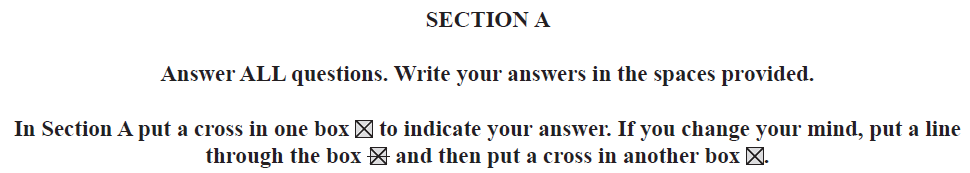
\includegraphics[width=19cm]{Exams/Section_A.png}
  
\end{center}

\vspace{30pt}

\begin{enumerate}
% Q1
    \item \quad Work out \hspace{3cm} \( \displaystyle \frac{1}{6} \) \, of \, \Large 48 

\vspace{110pt}

\begin{center}
\begin{tabular}{c@{\hspace{3cm}}c@{\hspace{3cm}}c@{\hspace{3cm}}c}
  6 & 8 & 40 & 288 \\
  
\includegraphics[width=0.5cm]{Exams/Cross_exams.png} & 
  
\includegraphics[width=0.5cm]{Exams/Cross_exams.png} & 
  
\includegraphics[width=0.5cm]{Exams/Cross_exams.png} & 
  
\includegraphics[width=0.5cm]{Exams/Cross_exams.png} \\
\end{tabular}
\end{center}

\hfill\raggedright (Total for Question 1 is 1 mark) 
\vspace{5pt}
\hline
\vspace{7pt}

% Q2
\item \quad What is the name given to this polygon? \\
\begin{center}
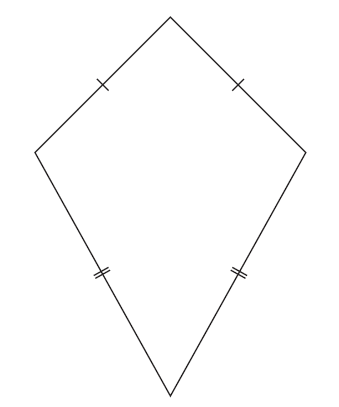
\includegraphics[width=6cm]{Exams/Kite.png}
\end{center}

\begin{center}
\begin{tabular}{c@{\hspace{3cm}}c@{\hspace{3cm}}c@{\hspace{3cm}}c}
  Kite & Parallelogram & Rectangle & Trapezium \\
  
\includegraphics[width=0.5cm]{Exams/Cross_exams.png} & 
  
\includegraphics[width=0.5cm]{Exams/Cross_exams.png} & 
  
\includegraphics[width=0.5cm]{Exams/Cross_exams.png} & 
  
\includegraphics[width=0.5cm]{Exams/Cross_exams.png} \\
\end{tabular}
\end{center}

\hfill\raggedright (Total for Question 2 is 1 mark) 
\vspace{5pt}
\hline
\vspace{7pt}

% Q3
\item \quad Work out \hspace{3cm} 874 - 298 
\vspace{90pt}

\begin{center}
\begin{tabular}{c@{\hspace{3cm}}c@{\hspace{3cm}}c@{\hspace{3cm}}c}
  572 & 574 & 576 & 624 \\
  
\includegraphics[width=0.5cm]{Exams/Cross_exams.png} & 
  
\includegraphics[width=0.5cm]{Exams/Cross_exams.png} & 
  
\includegraphics[width=0.5cm]{Exams/Cross_exams.png} & 
  
\includegraphics[width=0.5cm]{Exams/Cross_exams.png} \\
\end{tabular}
\end{center}

\hfill\raggedright (Total for Question 3 is 1 mark) 
\vspace{5pt}
\hline
\vspace{7pt}

% Q4
\item \quad John caught bus C from the shop to the school. 
\begin{center}
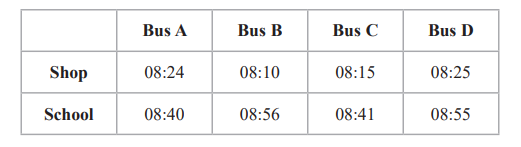
\includegraphics[width=13cm]{Year_6_Mixed_Tests/Bus_Timetable.png}
\end{center}

What time did he get to school? 

\vspace{15pt}

\begin{center}
\begin{tabular}{c@{\hspace{3cm}}c@{\hspace{3cm}}c@{\hspace{3cm}}c}
  08:15 & 08:40 & 08:41 & 08:55 \\
  
\includegraphics[width=0.5cm]{Exams/Cross_exams.png} & 
  
\includegraphics[width=0.5cm]{Exams/Cross_exams.png} & 
  
\includegraphics[width=0.5cm]{Exams/Cross_exams.png} & 
  
\includegraphics[width=0.5cm]{Exams/Cross_exams.png} \\
\end{tabular}
\end{center}

\hfill\raggedright (Total for Question 4 is 1 mark) 
\vspace{5pt}
\hline
\vspace{7pt}

% Q5 
\item \quad What is the range of these weights? 

\begin{center}
    98g \hspace{1cm} 83g \hspace{1cm} 44g \hspace{1cm} 67g \hspace{1cm} 140g \hspace{1cm} 98g \hspace{1cm} 65g 
\end{center}

\vspace{80pt}

\begin{center}
\begin{tabular}{c@{\hspace{3cm}}c@{\hspace{3cm}}c@{\hspace{3cm}}c}
  83g & 85g & 96g & 98g \\
  
\includegraphics[width=0.5cm]{Exams/Cross_exams.png} & 
  
\includegraphics[width=0.5cm]{Exams/Cross_exams.png} & 
  
\includegraphics[width=0.5cm]{Exams/Cross_exams.png} & 
  
\includegraphics[width=0.5cm]{Exams/Cross_exams.png} \\
\end{tabular}
\end{center}

\hfill\raggedright (Total for Question 5 is 1 mark) 
\vspace{5pt}
\hline
\vspace{7pt}

% Q6
\item \quad Work out \hspace{3cm} \( \displaystyle 8 + 3 \times 7 \)

\vspace{80pt}
\begin{center}
\begin{tabular}{c@{\hspace{3cm}}c@{\hspace{3cm}}c@{\hspace{3cm}}c}
  29 & 31 & 59 & 77 \\
  
\includegraphics[width=0.5cm]{Exams/Cross_exams.png} & 
  
\includegraphics[width=0.5cm]{Exams/Cross_exams.png} & 
  
\includegraphics[width=0.5cm]{Exams/Cross_exams.png} & 
  
\includegraphics[width=0.5cm]{Exams/Cross_exams.png} \\
\end{tabular}
\end{center}

\hfill\raggedright (Total for Question 6 is 1 mark) 
\vspace{5pt}
\hline
\vspace{7pt}

% Q7
\item \quad Which of these is a square number? 

\vspace{50pt}

\begin{center}
\begin{tabular}{c@{\hspace{3cm}}c@{\hspace{3cm}}c@{\hspace{3cm}}c}
  8 & 27 & 81 & 125 \\
  
\includegraphics[width=0.5cm]{Exams/Cross_exams.png} & 
  
\includegraphics[width=0.5cm]{Exams/Cross_exams.png} & 
  
\includegraphics[width=0.5cm]{Exams/Cross_exams.png} & 
  
\includegraphics[width=0.5cm]{Exams/Cross_exams.png} \\
\end{tabular}
\end{center}

\hfill\raggedright (Total for Question 7 is 1 mark) 
\vspace{5pt}
\hline
\vspace{7pt}

% Q8
\item \quad This shape is drawn on centimetre square paper. 

\begin{center}
    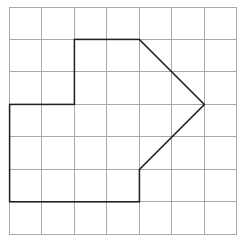
\includegraphics{Exams/Area_grid.png}
\end{center}

What is the area of this shape? 

\vspace{20pt}

\begin{center}
\begin{tabular}{c@{\hspace{3cm}}c@{\hspace{3cm}}c@{\hspace{3cm}}c}
  18 cm^{2} & 19 cm^{2} & 20 cm^{2} & 22 cm^{2} \\
  
\includegraphics[width=0.5cm]{Exams/Cross_exams.png} & 
  
\includegraphics[width=0.5cm]{Exams/Cross_exams.png} & 
  
\includegraphics[width=0.5cm]{Exams/Cross_exams.png} & 
  
\includegraphics[width=0.5cm]{Exams/Cross_exams.png} \\
\end{tabular}
\end{center}

\hfill\raggedright (Total for Question 8 is 1 mark) 
\vspace{5pt}
\hline
\vspace{7pt}

% Q9
\item \quad This clock shows the time a school finishes in the afternoon. 

\begin{center}
    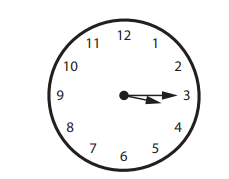
\includegraphics{Year_6_Mixed_Tests/Clock1.png}
\end{center}

How would this time be shown in 24-hour time? 

\vspace{20pt}

\begin{center}
\begin{tabular}{c@{\hspace{3cm}}c@{\hspace{3cm}}c@{\hspace{3cm}}c}
  03:45 & 13:15 & 15:00 & 15:15 \\
  
\includegraphics[width=0.5cm]{Exams/Cross_exams.png} & 
  
\includegraphics[width=0.5cm]{Exams/Cross_exams.png} & 
  
\includegraphics[width=0.5cm]{Exams/Cross_exams.png} & 
  
\includegraphics[width=0.5cm]{Exams/Cross_exams.png} \\
\end{tabular}
\end{center}

\hfill\raggedright (Total for Question 9 is 1 mark) 
\vspace{5pt}
\hline
\vspace{7pt}

% Q10
\item \quad Work out \hspace{3cm} \( \displaystyle 30 \% \) of \Large 120

\vspace{90}

\begin{center}
\begin{tabular}{c@{\hspace{3cm}}c@{\hspace{3cm}}c@{\hspace{3cm}}c}
  12 & 36 & 60 & 84  \\
  
\includegraphics[width=0.5cm]{Exams/Cross_exams.png} & 
  
\includegraphics[width=0.5cm]{Exams/Cross_exams.png} & 
  
\includegraphics[width=0.5cm]{Exams/Cross_exams.png} & 
  
\includegraphics[width=0.5cm]{Exams/Cross_exams.png} \\
\end{tabular}
\end{center}

\hfill\raggedright (Total for Question 10  is 1 mark) 
\vspace{5pt}
\hline
\vspace{7pt}

% Q11
\item \quad Which of these shapes has only one line of symmetry? 
\vspace{10}

\begin{center}
\begin{tabular}{c@{\hspace{1.5cm}}c@{\hspace{1.5cm}}c@{\hspace{1.5cm}}c}
  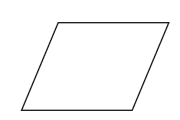
\includegraphics[width=3cm]{Exams/Rhombus.png} & 
  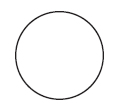
\includegraphics[width=3cm]{Exams/Circle.png} & 
  \includegraphics[width=3cm]{Exams/Square.png} & 
  \includegraphics[width=3cm]{Exams/Kite_2.png} \\
  
  \includegraphics[width=0.5cm]{Exams/Cross_exams.png} & 
  \includegraphics[width=0.5cm]{Exams/Cross_exams.png} & 
  \includegraphics[width=0.5cm]{Exams/Cross_exams.png} & 
  \includegraphics[width=0.5cm]{Exams/Cross_exams.png} \\
\end{tabular}
\end{center}

\hfill\raggedright (Total for Question 11  is 1 mark) 
\vspace{5pt}
\hline
\vspace{7pt}

% Q12
\item \quad Calculate \hspace{3cm} \( \displaystyle 6.4 \times 5 \) 

\vspace{120}

\begin{center}
\begin{tabular}{c@{\hspace{3cm}}c@{\hspace{3cm}}c@{\hspace{3cm}}c}
  32 & 64 & 128 & 320  \\
  \includegraphics[width=0.5cm]{Exams/Cross_exams.png} & 
  \includegraphics[width=0.5cm]{Exams/Cross_exams.png} & 
  \includegraphics[width=0.5cm]{Exams/Cross_exams.png} & 
  \includegraphics[width=0.5cm]{Exams/Cross_exams.png} \\
\end{tabular}
\end{center}

\hfill\raggedright (Total for Question 12  is 1 mark) 
\vspace{5pt}
\hline
\vspace{7pt}

% Q13
\item \quad What is 247517 rounded to the nearest ten thousand?  

\vspace{100}

\begin{center}
\begin{tabular}{c@{\hspace{3cm}}c@{\hspace{3cm}}c@{\hspace{3cm}}c}
  200,000 & 247,500 & 248,000 & 250,000  \\
  \includegraphics[width=0.5cm]{Exams/Cross_exams.png} & 
  \includegraphics[width=0.5cm]{Exams/Cross_exams.png} & 
  \includegraphics[width=0.5cm]{Exams/Cross_exams.png} & 
  \includegraphics[width=0.5cm]{Exams/Cross_exams.png} \\
\end{tabular}
\end{center}

\hfill\raggedright (Total for Question 13 is 1 mark) 
\vspace{5pt}
\hline
\vspace{7pt}

% Q14
\item \quad In a shop colouring pencils cost \textdollar 0.79 each. \\
\quad How much would it cost to buy 5 colouring pencils?
\vspace{120}

\begin{center}
\begin{tabular}{c@{\hspace{3cm}}c@{\hspace{3cm}}c@{\hspace{3cm}}c}
  \textdollar 2.37 & \textdollar 3.16 & \textdollar 3.95 & \textdollar 4.85  \\
  \includegraphics[width=0.5cm]{Exams/Cross_exams.png} & 
  \includegraphics[width=0.5cm]{Exams/Cross_exams.png} & 
  \includegraphics[width=0.5cm]{Exams/Cross_exams.png} & 
  \includegraphics[width=0.5cm]{Exams/Cross_exams.png} \\
\end{tabular}
\end{center}

\hfill\raggedright (Total for Question 14 is 1 mark) 
\vspace{5pt}
\hline
\vspace{7pt}

% Q15
    \item \quad Work out \hspace{3cm} \( \displaystyle \frac{5}{8} \) \, of \, \Large 240m 

\vspace{80pt}

\begin{center}
\begin{tabular}{c@{\hspace{3cm}}c@{\hspace{3cm}}c@{\hspace{3cm}}c}
  30m & 48m & 150m & 384m \\
  \includegraphics[width=0.5cm]{Exams/Cross_exams.png} & 
  \includegraphics[width=0.5cm]{Exams/Cross_exams.png} & 
  \includegraphics[width=0.5cm]{Exams/Cross_exams.png} & 
  \includegraphics[width=0.5cm]{Exams/Cross_exams.png} \\
\end{tabular}
\end{center}

\hfill\raggedright (Total for Question 15 is 1 mark) 
\vspace{5pt}
\hline
\vspace{7pt}

% Q16
\item \quad Jana’s class kept a record of how many students had a packed lunch each day for
a week. They displayed the information in this dual bar chart
%\vspace{5}

\begin{center}
\includegraphics[width=13cm]{Exams/Bar_Graph_Boys_Girls.png}
\end{center}

\vspace{5pt}

How many packed lunches in total did the girls have this week?

\vspace{10pt}

\begin{center}
\begin{tabular}{c@{\hspace{3cm}}c@{\hspace{3cm}}c@{\hspace{3cm}}c}
  130 & 240 & 250 & 490  \\
  \includegraphics[width=0.5cm]{Exams/Cross_exams.png} & 
  \includegraphics[width=0.5cm]{Exams/Cross_exams.png} & 
  \includegraphics[width=0.5cm]{Exams/Cross_exams.png} & 
  \includegraphics[width=0.5cm]{Exams/Cross_exams.png} \\
\end{tabular}
\end{center}

\hfill\raggedright (Total for Question 16 is 1 mark) 
\vspace{5pt}
\hline
\vspace{7pt}

% Q17
\item \quad Which one is a prime number? 

\vspace{30}

\begin{center}
\begin{tabular}{c@{\hspace{3cm}}c@{\hspace{3cm}}c@{\hspace{3cm}}c}
  51 & 53 & 57 & 52  \\
  \includegraphics[width=0.5cm]{Exams/Cross_exams.png} & 
  \includegraphics[width=0.5cm]{Exams/Cross_exams.png} & 
  \includegraphics[width=0.5cm]{Exams/Cross_exams.png} & 
  \includegraphics[width=0.5cm]{Exams/Cross_exams.png} \\
\end{tabular}
\end{center}

\hfill\raggedright (Total for Question 17 is 1 mark) 
\vspace{5pt}
\hline
\vspace{7pt}

% Q18
\item \quad Which one is a square number? 

\vspace{60}

\begin{center}
\begin{tabular}{c@{\hspace{3cm}}c@{\hspace{3cm}}c@{\hspace{3cm}}c}
  33 & 97 & 42 & 64  \\
  \includegraphics[width=0.5cm]{Exams/Cross_exams.png} & 
  \includegraphics[width=0.5cm]{Exams/Cross_exams.png} & 
  \includegraphics[width=0.5cm]{Exams/Cross_exams.png} & 
  \includegraphics[width=0.5cm]{Exams/Cross_exams.png} \\
\end{tabular}
\end{center}

\hfill\raggedright (Total for Question 18 is 1 mark) 
\vspace{5pt}
\hline
\vspace{7pt}

% Q19
\item \quad Which one is a cube number? 

\vspace{60}

\begin{center}
\begin{tabular}{c@{\hspace{3cm}}c@{\hspace{3cm}}c@{\hspace{3cm}}c}
  31 & 27 & 24 & 47  \\
  \includegraphics[width=0.5cm]{Exams/Cross_exams.png} & 
  \includegraphics[width=0.5cm]{Exams/Cross_exams.png} & 
  \includegraphics[width=0.5cm]{Exams/Cross_exams.png} & 
  \includegraphics[width=0.5cm]{Exams/Cross_exams.png} \\
\end{tabular}
\end{center}

\hfill\raggedright (Total for Question 19 is 1 mark) 
\vspace{5pt}
\hline
\vspace{7pt}

% Q20
\item \quad Abby has \textdollar 20. In a shop, a drink costs \textdollar 3.69 and a cake costs \textdollar 2.50 \\
\quad Abby buys a drink and two cakes. \\ 
\quad How much money does Abby have left?
\vspace{140}

\begin{center}
\begin{tabular}{c@{\hspace{3cm}}c@{\hspace{3cm}}c@{\hspace{3cm}}c}
  \textdollar 8.69 & \textdollar 11.31 & \textdollar 12.41 & \textdollar 13.81  \\
  \includegraphics[width=0.5cm]{Exams/Cross_exams.png} & 
  \includegraphics[width=0.5cm]{Exams/Cross_exams.png} & 
  \includegraphics[width=0.5cm]{Exams/Cross_exams.png} & 
  \includegraphics[width=0.5cm]{Exams/Cross_exams.png} \\
\end{tabular}
\end{center}

\hfill\raggedright (Total for Question 20 is 1 mark) 
\vspace{5pt}
\hline
\vspace{7pt}

\vspace{5pt}
\rule{\linewidth}{2pt} \\ 
\hfill\raggedright \textbf{TOTAL FOR SECTION A IS 20 MARKS} 
\vspace{5pt}

% Section B
\newpage

\begin{center}
\textbf{SECTION B} \\
\vspace{10pt}
\textbf{Answer all questions.}
\end{center}

% Q21
\item \quad Mr Jones asked his students what their favourite sport was.
He displayed their answers in this tally chart.

\begin{center}
\includegraphics[width=10cm]{Exams/Tallies_Sports_Mr_Jones.png}
\end{center}

(a) Complete the tally chart for this data. \hspace{6cm} (2)

\vspace{25pt}

(b) Construct a bar chart to represent this data. \hspace{4.65cm} (3)

\begin{center}
    Bar chart of favourite sports \\
    \includegraphics[width=13cm]{Exams/10_by_10_grid.png}
\end{center}

\vspace{15}

\hfill\raggedright (Total for Question 21 is 5 marks) 
\vspace{5pt}
\hline
\vspace{7pt}

% Q22
\item \quad (a) Work out \hspace{3cm} \( 4231 + 254 + 1309 \) \\ 
\vspace{130pt}
\hspace{15cm} .......... (1)

\quad (b) Work out \hspace{3cm} \( 3.43 + 15.31 + 20.42 \)  \\
\vspace{130pt}
\hspace{15cm} .......... (1) 

\vspace{10pt}

\hfill\raggedright (Total for Question 22 is 2 marks) 
\vspace{5pt}
\hline
\vspace{7pt}

% Q23
\item \quad (a) Calculate \hspace{3cm} \( \displaystyle 376.21 \times 10 \)
\vspace{120pt}
\hspace{15cm} .......... (1) 

\quad (b) Work out \hspace{3cm} \( \displaystyle 4903.2 \div 100 \) 
\vspace{120pt}
\hspace{15cm} .......... (1) 

\hfill\raggedright (Total for Question 23 is 2 marks) 
\vspace{5pt}
\hline
\vspace{7pt}

% Q24
\item \quad (a) Write \( \displaystyle \frac{18}{24} \) as a fraction in its simplest form.

\vspace{140pt} \\ 
\hspace{15cm} .......... (1) 

\quad (b) Work out \hspace{3cm} \( \displaystyle \Large 2 \frac{3}{5} + \frac{4}{5} \)
\vspace{140pt} \\
\hspace{15cm} .......... (1) 

\quad (c) Work out \hspace{3cm} \( \displaystyle \frac{1}{3} \times \frac{2}{5} \)
\vspace{110pt} \\
\hspace{15cm} .......... (1) 

\quad (d) Work out \hspace{3cm} \( \displaystyle \frac{1}{6} \div 5 \)
\vspace{110pt} \\
\hspace{15cm} .......... (1) 
\vspace{5pt}

 \hfill\raggedright (Total for Question 24 is 4 marks) 
\vspace{5pt}
\hline
\vspace{7pt}

% Q25
\item \quad Write these numbers in order of size. \\ 
\quad Start with the smallest.

\begin{center} 

\hspace{2cm} \( \displaystyle 2.36 \hspace{2cm} 3.26 \hspace{2cm} 2.6 \hspace{2cm} 2.63 \hspace{2cm} 2.3 \)
\vspace{100pt}

Smallest \quad ..... \hspace{2cm} ..... \hspace{2cm} ..... \hspace{2cm} ..... \hspace{2cm} ..... 

\end{center}

 \hfill\raggedright (Total for Question 25 is 2 marks) 
\vspace{5pt}
\hline
\vspace{7pt}

% Q26
\item \quad Here are the marks that Milan got in her maths assessments.
\begin{center}
\( \displaystyle 25 \hspace{1cm} 26 \hspace{1cm} 24 \hspace{1cm} 25 \hspace{1cm} 28 \hspace{1cm} 29 \hspace{1cm} 25 \)  \\ 
\end{center}
\quad What is the mean of Milan’s marks?

\vspace{120pt}
\hspace{15cm} .......... 
\vspace{5pt}

\hfill\raggedright (Total for Question 26 is 2 marks) 
\vspace{5pt}
\hline
\vspace{7pt}

% Q27
\item \quad What is the volume of this cuboid? \\ 
\vspace{5pt}

    \includegraphics[width=10cm]{Exams/Volume_1.png}

\vspace{20}
\hspace{15cm} ..........  
\vspace{5pt}

\hfill\raggedright (Total for Question 27 is 2 marks) 
\vspace{5pt}
\hline
\vspace{7pt}

% Q28 
\item \quad Calculate \hspace{2cm} \( \displaystyle 3408 \times 16 \) \hspace{2cm} You must show your working.  
\vspace{5pt}
% \quad \( \displaystyle 3408 \times 16 \) \\
% \vspace{5pt}
% \quad You must show your working. 

\vspace{150pt} 
\hspace{15cm} ..........  
\vspace{5pt}

\hfill\raggedright (Total for Question 28 is 2 marks) 
\vspace{5pt}
\hline
\vspace{7pt}

% Q29
\item \quad Calculate \hspace{2cm} \( \displaystyle 375 \div  4 \) \hspace{2cm} You must show your working.  
\vspace{5pt}

\vspace{150pt} 
\hspace{15cm} ..........  
\vspace{5pt}

\hfill\raggedright (Total for Question 29 is 2 marks) 
\vspace{5pt}
\hline
\vspace{7pt}

% Q30
\item \quad Calculate \hspace{2cm} \( \displaystyle 8432 \div  12 \) \hspace{2cm} You must show your working.  
\vspace{5pt}

\vspace{150pt} 
\hspace{15cm} ..........  
\vspace{5pt}

\hfill\raggedright (Total for Question 30 is 2 marks) 
\vspace{5pt}
\hline
\vspace{7pt}

%Q31
\item \quad Write \textit{\textbf{five million, three hundred and four thousand, five hundred and one}} in digits. 

 \vspace{60pt}
 \hspace{13cm} ..............................

 \vspace{5pt}

\hfill\raggedright (Total for Question 31 is 2 mark) 
\vspace{7pt}
\hline
\vspace{7pt}

% Q32
 \item \quad Write \bm{\mathit{573002}} in words.

 \vspace{30pt}

\noindent \dotuline{\hspace{18cm}} \\
\vspace{7pt}
\noindent \dotuline{\hspace{18cm}} \\
\vspace{7pt}

\hfill\raggedright (Total for Question 32 is 2 mark) 
\vspace{7pt}
\hline
\vspace{7pt}

% Q33
\item \quad \text{ Fill in A, B, C and D in the number line below. } % \hspace{2cm} [2 marks]
\vspace{10pt}

% Negative number line 

\begin{tikzpicture}[x=0.8cm]  % Set the x unit vector length to 0.8cm
    % Draw the main line
    \draw[->] (-10,0) -- (10,0);
    
    % Draw tick marks and labels
    \foreach \x in {-10, -8, ..., 10} {
        \draw (\x,-0.1) -- (\x,0.1);
        % Omit labels at positions -7, -3, 2, and 8 to leave them blank for letters
        \ifnum\x=-8 \else \ifnum\x=-6 \else \ifnum\x=-2 \else 
        \ifnum\x=2 \else \ifnum\x=4 \else  \ifnum\x=8 \else 
            \node[below] at (\x,-0.2) {$\x$};
        \fi\fi\fi\fi\fi\fi
    }
    
    % Draw letters 'A', 'B', 'C', and 'D' at positions -7, -3, 2, and 8
    \node[below] at (-8,-0.2) {A};
    \node[below] at (-2,-0.2) {B};
    \node[below] at (4,-0.2) {C};
   % \node[below] at (8,-0.2) {D};
    
\end{tikzpicture}
\vspace{70pt}
\begin{center}
    A ..... \hspace{2cm} B ..... \hspace{2cm} C ..... \hspace{2cm} D .....
\end{center}

\hfill\raggedright (Total for Question 33 is 2 marks) 
\vspace{5pt}
\hline
\vspace{7pt}

% Q34
\item \text{ Write these numbers in order of size. Start with the smallest. } %\hspace{2cm} [2 marks] 
\begin{center}
\hspace{2cm} 5.06 \hspace{2cm} \( \displaystyle \frac{5}{6}\) \hspace{2cm} 56\% \hspace{2cm} 5.006 
\vspace{100pt}

Smallest .......\hspace{2cm}.....\hspace{2cm}.....\hspace{2cm}.....\hspace{2cm} \\
\end{center}

\hfill\raggedright (Total for Question 34 is 2 marks) 
\vspace{5pt}
\hline
\vspace{7pt}

% Q35
\item \quad The figure below is Mwago's paper plan for building a house.  

\begin{center}
\includegraphics[width=7cm]{Exams/cs_1.png} 
\end{center}
\\

\quad (a) Find its perimeter.
\vspace{170pt} \\
\hspace{15cm} .......... (2)  
\vspace{5pt}

\\
\quad (b) Find its area. 
\vspace{180pt} \\
\hspace{15cm} ..........(2)  
\vspace{5pt}

\hfill\raggedright (Total for Question 35 is 4 marks) 
\vspace{5pt}
\hline
\vspace{7pt}

% Q36
\item \quad 240 students were asked how they travelled to school. \\
\quad 25\% came by car. \\ 
\quad 30\% came by bus. \\
\quad The remaining students walked to school. \\

\vspace{10pt}
\quad Shirleen says
\begin{center}
\textit{‘more than 100 students walked to school’}
\end{center}
\vspace{10pt}

\quad Is Shirleen correct? \\
\quad You must show your working.

\vspace{200pt} 
% \hspace{15cm} ..........  
%\vspace{5pt}

\hfill\raggedright (Total for Question 36 is 3 marks) 
\vspace{5pt}
\hline
\vspace{7pt}

\vspace{5pt}
\rule{\linewidth}{2pt} \\ 
\hfill\raggedright \textbf{TOTAL FOR SECTION B IS 40 MARKS}  \\
\hfill\raggedright \textbf{TOTAL FOR PAPER IS 60 MARKS} \\
\vspace{90pt}


\hspace{8cm} \textbf{The End}


\end{enumerate}

\end{document}

 